\chapter{Expression des besoins}
\clearpage
\section{introduction}

L'objectif de ce projet est de développer un logiciel de gestion des ressources humaines (RH) pour l'Agence Nationale de Régulation de la Commande Publique (ARCOP). Ce logiciel permettra de centraliser et d'automatiser la gestion des congés, des absences, des formations, et des évaluations des employés, en s'adressant directement aux employés et au département de la Gestion des Ressources Humaines (GRH).
\section{Spécifications}
\subsection{Spécifications Fonctionnelles}


\subsubsection{Gestion des Congés et Absences}
\begin{itemize}
    \item \textbf{Mise à jour du planning et du solde des congés :} Le logiciel doit permettre aux employés de l'ARCOP de demander des congés en ligne, avec une mise à jour du planning et du solde de congés. Les demandes seront soumises au supérieur, puis au DG après approbation du GRH.

    
    \item \textbf{Rapports personnalisables :} Le logiciel offrira la possibilité de générer des rapports sur la durée, la fréquence, et les motifs des congés, personnalisables selon les besoins du GRH.
    

    
  
\end{itemize}

\subsubsection{Gestion des dossiers}
\begin{itemize}
    \item \textbf{Dossier personnalisé en ligne pour chaque agent :} Un dossier en ligne pour chaque employé de l'ARCOP sera accessible via la version web du logiciel, contenant toutes les informations concernant ses congés, absences, et autres données RH.
    
    \item \textbf{Téléchargement des bulletins de paie :} Extraction des bulletins de paie depuis Sage Paie, puis les rendre disponibles aux employés dans l'application après un chargement.
    \item \textbf{Demande de documents administratifs :} Les employés
    pourront demander des documents administratifs en ligne, tels que des attestations de travail, des certificats de travail.
\end{itemize}

\subsubsection{Publication des notes et informations}
\begin{itemize}
    \item \textbf{Publication des notes et informations :} Le GRH pourra publier des notes, des informations, et des documents RH pour les employés, accessibles via l'interface web du logiciel.
    \item \textbf{Alertes et notifications :} Les employés recevront des alertes et des notifications pour les rappeler des échéances, des actions sur les demandes.
\end{itemize}

\subsection{Spécifications techniques}

\subsubsection{Langages et Technologies}
\begin{itemize}
    \item \textbf{Framework :} Laravel pour une gestion efficace de la logique serveur et du backend.
    \item \textbf{Base de données :} MySQL ou PostgreSQL pour la gestion des données avec Eloquent ORM.
    \item \textbf{Frontend :} Blade pour une interface utilisateur dynamique et fluide.

\end{itemize}


\subsubsection{Sécurité}
\begin{itemize}
    \item Chiffrement des données sensibles.
    \item Gestion des accès par rôles.
\end{itemize}

\subsubsection{Hébergement}
\begin{itemize}
    \item Déploiement sur les serveurs internes de l'ARCOP.
\end{itemize}
\subsection{Exigences non fonctionnelles}


\subsubsection{Fiabilité}
\begin{itemize}
    \item Le logiciel doit être disponible 99.9\% du temps, excluant les périodes de maintenance planifiée.
    \item Les données doivent être sauvegardées quotidiennement avec une possibilité de restauration en cas de panne.
\end{itemize}

\subsubsection{Utilisabilité}
\begin{itemize}
    \item L'interface utilisateur doit être intuitive et facile à utiliser, avec une courbe d'apprentissage minimale.
    \item Une documentation utilisateur complète doit être fournie, incluant des guides et des tutoriels.
\end{itemize}

\subsubsection{Compatibilité}
\begin{itemize}
    \item \textbf{Navigateurs :} Le logiciel doit être compatible avec les dernières versions de Chrome, Firefox, Safari, et Edge.
    \item \textbf{Mobile :} L'application web doit être responsive et accessible depuis les navigateurs mobiles.
\end{itemize}

\subsubsection{Scalabilité}
Le logiciel doit pouvoir gérer un nombre croissant d'utilisateurs et de données sans dégradation des performances.


\subsubsection{Nom du logicièl}
Le logiciel sera nommé \textbf{OptiHR}, un nom qui allie modernité et professionnalisme, reflétant une gestion
optimale des ressources humaines.


\section{Définition des acteurs systèmes}
Le logiciel est destiné aux employés de l’ARCOP et au département de la Gestion des Ressources Humaines (GRH), facilitant une gestion efficace des congés, de la formation, et des évaluations.
Les utilisateurs principaux du systemes sont:
\begin{itemize}
    \item Employé 
    \item GRH 
    \item DSAF 
    \item DG 
\end{itemize}
\subsection{Employé}
L'utilisateur \textbf{Employé} désignent un employé de l'ARCOP. Il utilisent le logiciel pour demander des congés, demander des documents, suivre des formations, et participer aux évaluations. Ils accèdent à leur dossier personnel en ligne pour consulter leur solde de congés, leurs absences, et leurs évaluations.
\subsection{GRH}
Le \textbf{GRH} désigne le \textbf{Chef division des ressources humaines et services généraux} de l'ARCOP. Il utilise le logiciel pour gérer les demandes de congés,les documents, les formations, et les évaluations des employés. Il peut consulter les rapports RH, planifier les entretiens,publier des notes ou informations, et suivre les indicateurs de performance.
\subsection{DSAF }
Le \textbf{DSAF} désigne le \textbf{ Directeur des services administratif et financier} de l'ARCOP. Il utilise le logiciel pour suivre les demandes effectuées par les employées. IL interagite principallement en consultation.
\subsection{DG}
Le \textbf{DG} désigne le \textbf{Directeur Général} de l'ARCOP. Il utilise le logiciel pour valider les demandes de congés, les budgets de formation, et les résultats des évaluations. Il peut consulter les rapports RH et financiers pour prendre des décisions stratégiques en matière de ressources humaines.


\section{D\'efinition des cas d'utilisation}

Un diagramme de cas d'utilisation est une représentation graphique des interactions entre les acteurs d'un système et ses fonctionnalités. Il permet d'identifier et de structurer les besoins fonctionnels du logiciel en décrivant les actions réalisées par chaque acteur. Ce type de diagramme est particulièrement utile pour comprendre les interactions des utilisateurs avec le système et pour définir clairement les responsabilités de chaque acteur.

Dans ce contexte, nous définissons les cas d'utilisation pour chaque fonctionnalités énoncés précédemment.
\subsection{Gestion des Congés et Absences}
\subsubsection{Description de la fonctionnalité}
La gestion des congés et des absences est une fonctionnalité essentielle du logiciel, permettant aux employés de demander des congés en ligne, de consulter leur solde de congés, et de générer des rapports sur les congés et les absences.
\subsubsection{Description des cas d'utilisation}
\begin{itemize}
    \item \textbf{Demande de congé :} L'employé peut demander un congé en ligne, en précisant la date, la durée, et le motif.
    \item \textbf{Annulation de la demande de congé :} L'employé peut annuler sa demande de congé en ligne tant que son supérieur hiérarchique n'a pas encore effectué d'action.
    \item \textbf{approbation du supérieur :} Le supérieur hiérarchique peut valider ou refuser la demande de congé de l'employé.
    \item \textbf{Approbation du GRH :} Le GRH peut valider ou refuser la demande de congé après approbation du supérieur.
    \item \textbf{Validation du DG :} Le DG peut valider ou refuser la demande de congé après approbation du GRH.
    \item \textbf{Consultation du solde de congés :} L'employé peut consulter son solde de congés et les congés déjà pris.
    \item \textbf{Génération de rapports :} Le GRH peut générer des rapports sur les congés, les absences, et les motifs.
    \item \textbf{Télécharger le document de validation :} L'employé peut télécharger le pdf de validation de la demande de congés ou absences.
\end{itemize}
\subsubsection{Diagramme de cas d'utilisation}
\begin{figure}[H]
    \centering
    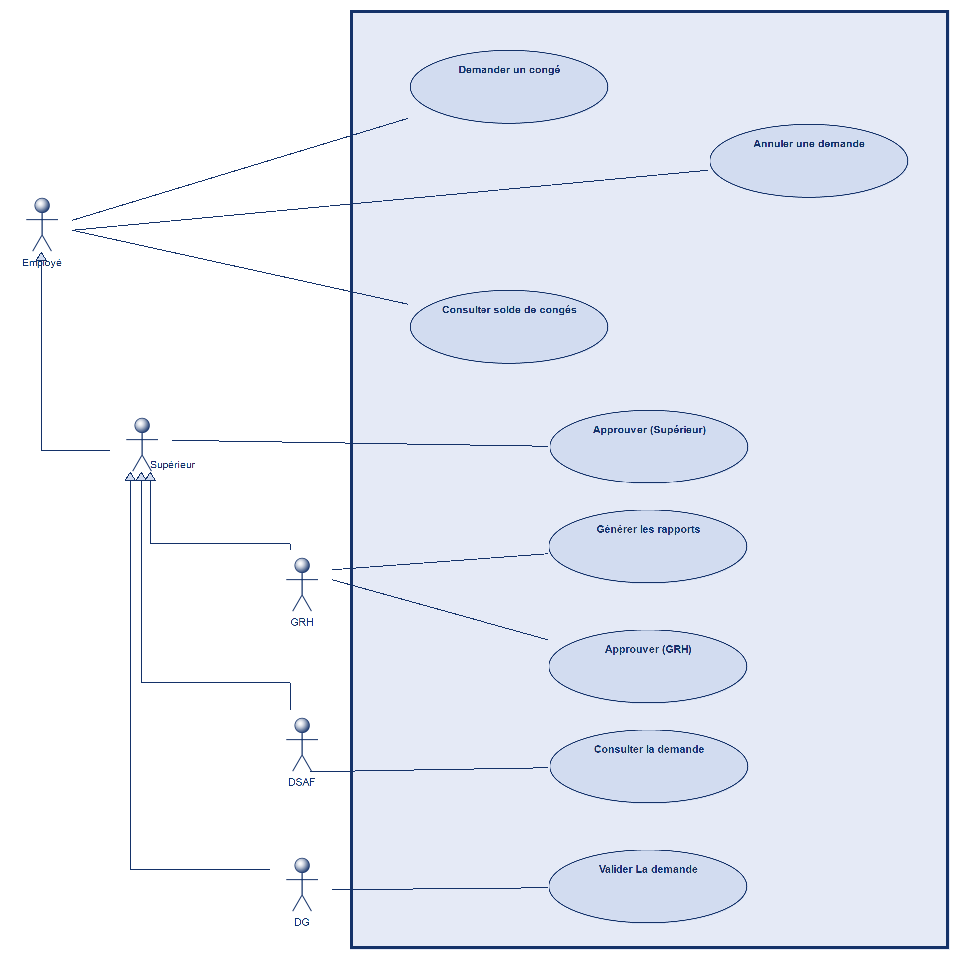
\includegraphics[width=0.8\textwidth]{images/diagrammes/use-cases/conges.png}
    \caption{Diagramme de cas d'utilisation Gestion des Congés et Absences}
    \label{fig:use_case_gestion_conges}

\end{figure}
\subsubsection{Diagramme de processus}
Le diagramme de processus modélise les étapes d'exécution de certaines fonctionnalités clés du système. Le diagramme de processus pour la gestion des congés et des absences est le suivant :
\begin{figure}[H]
    \centering
    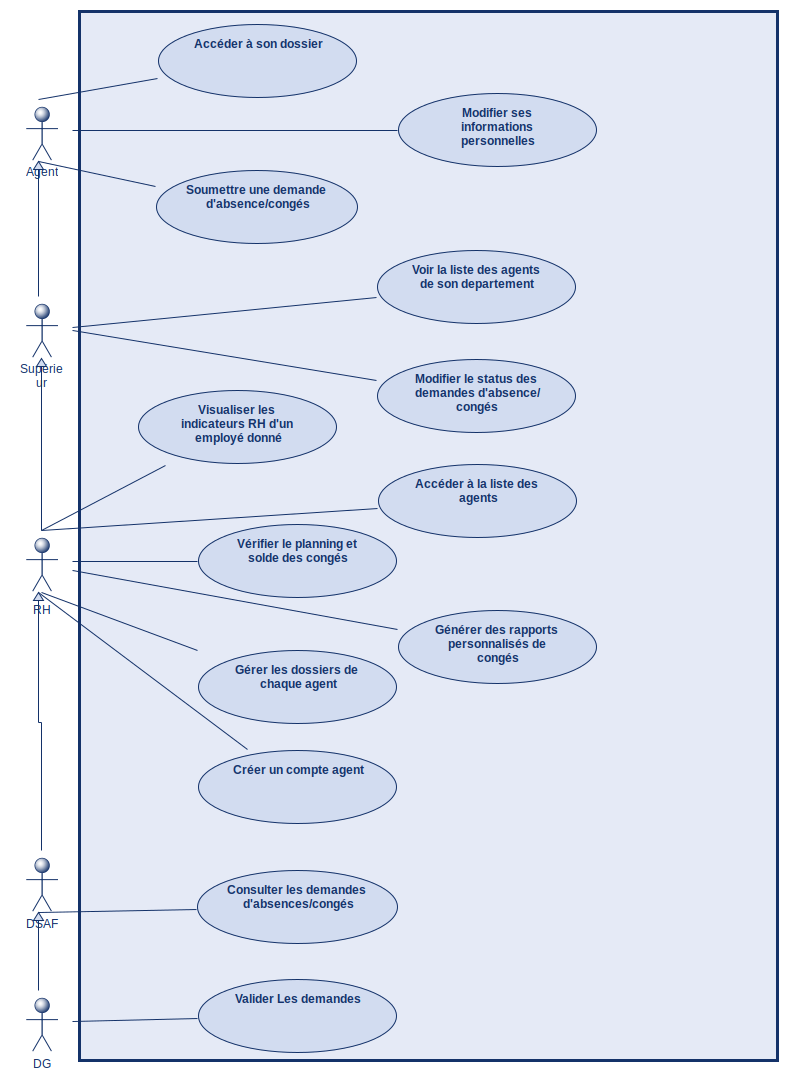
\includegraphics[width=0.8\textwidth]{images/diagrammes/flowcharts/conges.png}
    \caption{Diagramme de processus Gestion des Congés et Absences}
    \label{fig:flow_gestion_conges}
\end{figure}

\subsection{Gestion des dossiers}
\subsubsection{Description de la fonctionnalité}
La gestion des dossiers permet aux employés de consulter leur dossier personnel en ligne, de télécharger des bulletins de paie, et de demander des documents administratifs.
\subsubsection{Description des cas d'utilisation}
\begin{itemize}
    \item \textbf{Consultation du dossier personnel :} L'employé peut consulter son dossier personnel en ligne, contenant ses congés, absences, formations, et évaluations.
    \item \textbf{Téléchargement des bulletins de paie :} L'employé peut télécharger ses bulletins de paie depuis l'application.
    \item \textbf{Demande de documents administratifs :} L'employé peut demander des documents administratifs en ligne, tels que des attestations de travail, des certificats de travail.
\end{itemize}
\subsubsection{Diagramme de cas d'utilisation}
\begin{figure}[H]
    \centering
    \includegraphics[width=0.8\textwidth]{images/diagrammes/use-cases/dossiers.png}
    \caption{Diagramme de cas d'utilisation Gestion des dossiers}
    \label{fig:use_case_gestion_dossiers}
\end{figure}
\subsubsection{Diagramme de processus}
Le diagramme de processus pour la gestion des dossiers est le suivant :
\begin{figure}[H]
    \centering
    \includegraphics[width=0.8\textwidth]{images/diagrammes/flowcharts/dossiers.png}
    \caption{Diagramme de processus Gestion des dossiers}
    \label{fig:flow_gestion_dossiers}
\end{figure}
\subsection{Publication des notes et informations}
\subsubsection{Description de la fonctionnalité}
La publication des notes et des informations permet au GRH de publier des notes, des informations, et des documents RH pour les employés, avec des alertes et des notifications pour les rappeler des échéances.
\subsubsection{Description des cas d'utilisation}   
\begin{itemize}
    \item \textbf{Publication des notes et informations :} Le GRH peut publier des notes, des informations, et des documents RH pour les employés.
    \item \textbf{Alertes et notifications :} Les employés reçoivent des alertes et des notifications pour les rappeler des échéances, des actions sur les demandes.
\end{itemize}
\subsubsection{Diagramme de cas d'utilisation}
\begin{figure}[H]
    \centering
    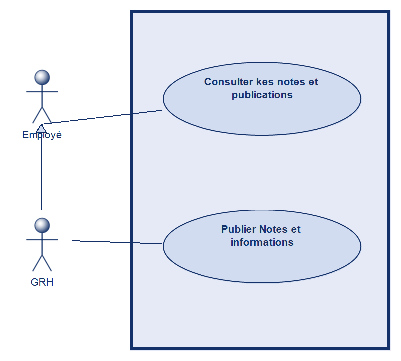
\includegraphics[width=0.8\textwidth]{images/diagrammes/use-cases/note.png}
    \caption{Diagramme de cas d'utilisation Publication des notes et informations}
    \label{fig:use_case_publication}
\end{figure}
\subsubsection{Diagramme de processus}
Le diagramme de processus pour la publication des notes et des informations est le suivant :
\begin{figure}[H]
    \centering
    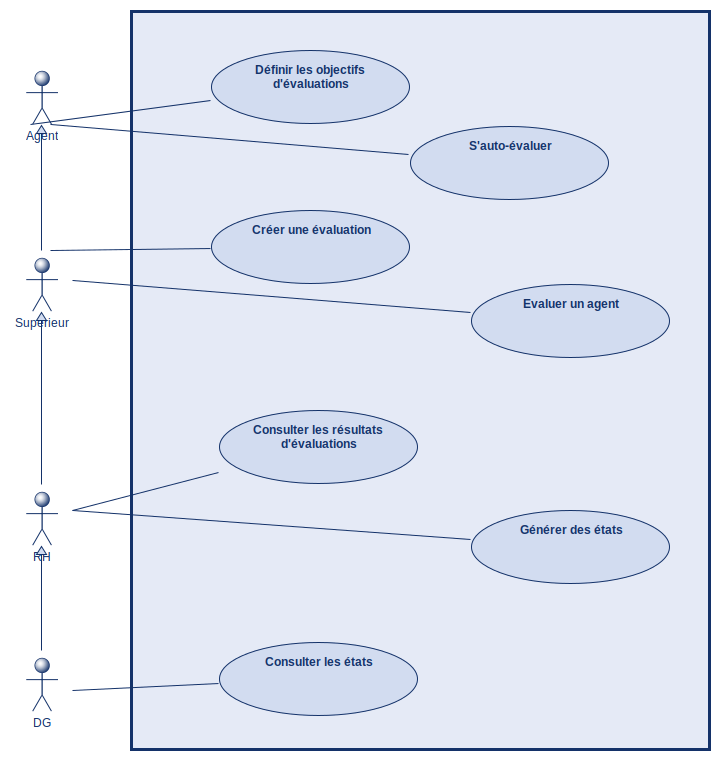
\includegraphics[width=0.8\textwidth]{images/diagrammes/flowcharts/note.png}
    \caption{Diagramme de processus Publication des notes et informations}
    \label{fig:flow_publication}
\end{figure}

\section{Conclusion}
Ce cahier des charges définit les fonctionnalités et les exigences techniques d'un logiciel de gestion RH performant et sécurisé pour l'ARCOP. Le logiciel, nommé \textbf{OptiHR}, répondra aux besoins spécifiques du GRH et des employés, en facilitant la gestion des congés, des formations, et des évaluations, d'éditer les bulletins de paie tout en étant évolutif et intégrable aux systèmes existants. La prochaine étape consistera à concevoir l'architecture du système et à élaborer les diagrammes UML pour modéliser les interactions entre les différents modules.
\clearpage
